%Este trabalho está licenciado sob a Licença Atribuição-CompartilhaIgual 4.0 Internacional Creative Commons. Para visualizar uma cópia desta licença, visite http://creativecommons.org/licenses/by-sa/4.0/deed.pt_BR ou mande uma carta para Creative Commons, PO Box 1866, Mountain View, CA 94042, USA.

\chapter{Redes Informadas pela Física}\label{cap_pinns}
\thispagestyle{fancy}
[[tag:construcao]]

\hlemph{Redes neurais informadas pela física} (PINNs, do inglês, \textit{physics-informed neural networks}) são métodos de \textit{deep learning} para a solução de equações diferenciais.

% \section{Problemas de Valores Iniciais}
% [[tag:construcao]]

% Consideramos um \hlemph{problema de valor inicial} (\hlemph{IVP}, do inglês, \textit{initial value problem})
% \begin{subequations}\label{eq:ivp}\hleq
%   \begin{align}
%     &y'(t) = g\left(t, y(t)\right), ~t_0 < t < t_f,\\
%     &y(t_0) = y_0,
%   \end{align}
% \end{subequations}
% com dada $g:\mathbb{R}^2\to\mathbb{R}$ e dados valor inicial $y_0\in\mathbb{R}$, tempos inicial $t_0\in\mathbb{R}$ e final $t_f\in\mathbb{R}$.

% \subsection{Euler PINN}
% [[tag:construcao]]

% A solução do IVP \eqref{eq:ivp} pode ser obtida por uma \hlemph{rede neural informada pela física} (PINN, do inglês, \textit{physics-informed neural network}) assumindo a seguinte aproximação de \href{https://notaspedrok.com.br/notas/MatematicaNumericaII/cap_pvi_sec_euler.html}{Euler explícita}
% \begin{subequations}\label{eq:ivp}\hleq
%   \begin{align}
%     &y^{(s+1)} = y^{(s)} + h_tg\left(t^{(s)}, y^{(s)}\right), ~0\leq s\leq n_t-1,\\
%     &y^{(0)} = y_0,
%   \end{align}
% \end{subequations}
% onde $y^{(s)} \approx y\left(t^{(s)}\right)$, nos tempos discretos $t^{(s)} = t_0 + sh_t$, com passo $h_t=(t_t-t_0)/n_t$, $s = 0, 1, 2, \dotsc, n_t$.

% Nosso modelo PINN é uma \href{https://notaspedrok.com.br/notas/RedesNeuraisArtificiais/cap_mlp_sec_modelo.html}{perceptron multicamada} (MLP)
% \begin{equation}\hleq
%   \tilde{y} = \mathcal{N}\left(t; \left\{W^{(l)}, \pmb{b}^{(l)}, \pmb{f}^{(l)}\right\}_{l=1}^{n_h+1}\right),
% \end{equation}
% de dada arquitetura $1 - n_n\times n_h - 1$, i.e. uma entrada, $n_h$ camadas escondidas, cada com $n_n$ neurônios e uma saída. A entrada é o valor do tempo $t$ e a saída é $\tilde{y} = \mathcal{N}(t) \approx y(t)$, a estimativa da solução do IVP \eqref{eq:ivp}. Escolhidas as funções de ativação $\pmb{f}^{(l)}$, $l = 1, 2, \dotsc, n_h+1$, o treinamento da PINN consiste em resolver o seguinte problema de minimização
% \begin{equation}\hleq
%   \min_{\left\{W^{(l)}, \pmb{b}^{(l)}\right\}_{l=1}^{n_h+1}} \frac{1}{n_s}\sum_{s=0}^{n_s-1}\left|\mathcal{R}^{(s)}\right|^2 + p_p\left|\tilde{y}^{(0)} - y_0\right|^2,
% \end{equation}
% onde $p_p>0$ é um dado \hlemph{parâmetro de penalização} e $\mathcal{R}^{(s)}$ é o \hlemph{resíduo}
% \begin{equation}\hleq
%   \mathcal{R}^{(s)} := \frac{y^{(s+1)} - y^{(s)}}{h_t} - h_tg\left(t^{(s)}, y^{(s)}\right).
% \end{equation}

% \begin{ex}
%   Consideramos o seguinte IVP
%   \begin{subequations}
%     \begin{align}
%       &y'(t) = \sin(t) - y, ~0 < t < 1,\\
%       &y(0) = \frac{1}{2}.
%     \end{align}
%   \end{subequations}
% \end{ex}

% \begin{lstlisting}[caption=pyEulerPINN.py]
% import torch
% from scipy.integrate import quad

% # model
% ## num hidden layers
% nh = 2
% ## num neurons per hidden layer
% nn = 50
% ## activation fun in hidden layers
% fh = torch.nn.Tanh()
% ## model architecture
% model = torch.nn.Sequential()
% model.add_module('layer_1', torch.nn.Linear(1,nn))
% model.add_module('fun_1', fh)
% for l in range(2, nh):
%     model.add_module(f'layer_{l}', torch.nn.Linear(nn,nn))
%     model.add_module(f'fun_{l}', fh)
% model.add_module(f'layer_{nh}', torch.nn.Linear(nn,1))

% # IVP params

% ## init time
% t0 = 0.
% ## init condition
% y0 = 0.5
% ## final time
% tf = 1.

% ## num of time samples
% ns = 10
% ## time step
% ht = (tf - t0)/ns
% ## time samples
% ts = torch.linspace(t0, tf, ns+1).reshape(-1,1)

% ## rhs
% def g(t, y):
%     return y + torch.sin(t)

% # training
% ## num of epochs
% nepochs = 10000
% ## output loss freq
% eout = 100
% ## tolerance
% tol = 1e-4
% ## early-stop
% n_iter_no_change = 100

% ## optimizer
% optim = torch.optim.Adam(model.parameters(), lr=1e-3)

% # training loop
% count_no_change = 0
% best_loss = 1e38
% for epoch in range(nepochs):

%     # forward
%     yy = model(ts)

%     # loss
%     ## t>0
%     lup = torch.mean(((yy[1:] - yy[:-1])/ht \
%                       - g(ts[:-1], yy[:-1]))**2)
%     ## t = 0
%     lic = (yy[0] - y0)**2

%     loss_train = lup + lic        

%     # backward
%     optim.zero_grad()
%     loss_train.backward()
%     optim.step()

%     # validation
%     ys = model(ts).detach()
%     yv = torch.empty_like(ys)
%     yv[0] = y0
%     for s in range(1,ns+1):
%         yv[s] = yv[s-1] + quad(lambda t: g(torch.tensor([[t]]),
%                                       model(torch.tensor([[t]])).detach()),
%                                ts[s-1], ts[s])[0]
%     loss_valid = torch.mean((ys - yv)**2)

%     if (loss_valid < best_loss):
%         torch.save(model, 'model.pt')
%         best_loss = loss_valid
%         count_no_change = 0
%     else:
%         count_no_change += 1

%     if ((epoch % eout == 0) or (count_no_change == 0)):
%         msg = f'{epoch}: train = {loss_train.item():.4e}, valid = {loss_valid.item():.4e}'
%         if (count_no_change == 0):
%             msg += ' (best)'
%         print(msg)

%     if ((best_loss < tol) or (count_no_change > n_iter_no_change)):
%         break

%     if (loss_train < tol):
%         break
% \end{lstlisting}

% \subsection{AD-PINN}
% [[tag:construcao]]

% Aqui nosso modelo PINN é novamnte uma \href{https://notaspedrok.com.br/notas/RedesNeuraisArtificiais/cap_mlp_sec_modelo.html}{perceptron multicamada} (MLP)
% \begin{equation}\hleq
%   \tilde{y} = \mathcal{N}\left(t; \left\{W^{(l)}, \pmb{b}^{(l)}, \pmb{f}^{(l)}\right\}_{l=1}^{n_h+1}\right),
% \end{equation}
% de dada arquitetura $1 - n_n\times n_h - 1$, i.e. uma entrada, $n_h$ camadas escondidas, cada com $n_n$ neurônios e uma saída. A entrada é o valor do tempo $t$ e a saída é $\tilde{y} = \mathcal{N}(t) \approx y(t)$, a estimativa da solução do IVP \eqref{eq:ivp}. Escolhidas as funções de ativação $\pmb{f}^{(l)}$, $l = 1, 2, \dotsc, n_h+1$, o treinamento da PINN consiste em resolver o seguinte problema de minimização
% \begin{equation}\hleq
%   \min_{\left\{W^{(l)}, \pmb{b}^{(l)}\right\}_{l=1}^{n_h+1}} \frac{1}{n_s}\sum_{s=0}^{n_s-1}\left|\mathcal{R}^{(s)}\right|^2 + p_p\left|\tilde{y}^{(0)} - y_0\right|^2,
% \end{equation}
% onde $p_p>0$ é um dado \hlemph{parâmetro de penalização} e $\mathcal{R}^{(s)}$ é o \hlemph{resíduo}
% \begin{equation}\hleq
%   \mathcal{R}^{(s)} := y'^{(s)} - h_tg\left(t^{(s)}, y^{(s)}\right),
% \end{equation}
% com $y'^{(s)} \approx y'\left(t^{(s)}\right)$ computada por diferenciação automática da MLP.

% \begin{ex}
%   Consideramos o seguinte IVP
%   \begin{subequations}
%     \begin{align}
%       &y'(t) = \sin(t) - y, ~0 < t < 1,\\
%       &y(0) = \frac{1}{2}.
%     \end{align}
%   \end{subequations}
% \end{ex}

% \begin{lstlisting}[caption=pyEulerPINN.py]
% import torch
% from scipy.integrate import quad

% # model
% ## num hidden layers
% nh = 2
% ## num neurons per hidden layer
% nn = 50
% ## activation fun in hidden layers
% fh = torch.nn.Tanh()
% ## model architecture
% model = torch.nn.Sequential()
% model.add_module('layer_1', torch.nn.Linear(1,nn))
% model.add_module('fun_1', fh)
% for l in range(2, nh):
%     model.add_module(f'layer_{l}', torch.nn.Linear(nn,nn))
%     model.add_module(f'fun_{l}', fh)
% model.add_module(f'layer_{nh}', torch.nn.Linear(nn,1))

% # IVP params

% ## init time
% t0 = 0.
% ## init condition
% y0 = 0.5
% ## final time
% tf = 1.

% ## num of time samples
% ns = 10
% ## time step
% ht = (tf - t0)/ns
% ## time samples
% ts = torch.linspace(t0, tf, ns+1).reshape(-1,1)

% ## rhs
% def g(t, y):
%     return y + torch.sin(t)

% # training
% ## num of epochs
% nepochs = 10000
% ## output loss freq
% eout = 100
% ## tolerance
% tol = 1e-4
% ## early-stop
% n_iter_no_change = 100

% ## optimizer
% optim = torch.optim.Adam(model.parameters(), lr=1e-3)

% # training loop
% count_no_change = 0
% best_loss = 1e38
% for epoch in range(nepochs):

%     # forward
%     yy = model(ts)

%     # loss
%     ## t>0
%     lup = torch.mean(((yy[1:] - yy[:-1])/ht \
%                       - g(ts[:-1], yy[:-1]))**2)
%     ## t = 0
%     lic = (yy[0] - y0)**2

%     loss_train = lup + lic        

%     # backward
%     optim.zero_grad()
%     loss_train.backward()
%     optim.step()

%     # validation
%     ys = model(ts).detach()
%     yv = torch.empty_like(ys)
%     yv[0] = y0
%     for s in range(1,ns+1):
%         yv[s] = yv[s-1] + quad(lambda t: g(torch.tensor([[t]]),
%                                       model(torch.tensor([[t]])).detach()),
%                                ts[s-1], ts[s])[0]
%     loss_valid = torch.mean((ys - yv)**2)

%     if (loss_valid < best_loss):
%         torch.save(model, 'model.pt')
%         best_loss = loss_valid
%         count_no_change = 0
%     else:
%         count_no_change += 1

%     if ((epoch % eout == 0) or (count_no_change == 0)):
%         msg = f'{epoch}: train = {loss_train.item():.4e}, valid = {loss_valid.item():.4e}'
%         if (count_no_change == 0):
%             msg += ' (best)'
%         print(msg)

%     if ((best_loss < tol) or (count_no_change > n_iter_no_change)):
%         break

%     if (loss_train < tol):
%         break
% \end{lstlisting}

% \subsection{Exercícios}
% [[tag:construcao]]

\section{Aplicação: Equação de Poisson}\label{cap_mlp_sec_eqpoisson}

Vamos criar uma \hl{MLP para resolver o problema de Poisson}{\poisson}
\begin{subequations}\label{cap_mlp_sec_eqlaplace:eq:prob}
  \begin{align}
    &\hleq -\Delta u = f, ~\pmb{x}\in \mathcal{D} = (-1, 1)^2,\label{cap_mlp_sec_eqpoisson:eq:eqPossion}\\
    &\hleq u = 0, ~\pmb{x}\in\p D,\label{cap_mlp_sec_eqpoisson:eq:cc}
  \end{align}
\end{subequations}
com fonte dada
\begin{equation}
  f(x_1, x_2) = \pi^2\sen(\pi x_1)\sen(\pi x_2).
\end{equation}

No treinamento, vamos usar a \hl{função erro baseada no resíduo da equação de Poisson} \eqref{cap_mlp_sec_eqpoisson:eq:eqPossion} \hl{e nas condições de contorno} \eqref{cap_mlp_sec_eqpoisson:eq:cc}. Mais especificamente, assumimos a função erro
\begin{equation}\hleq
  \varepsilon := \underbrace{\frac{1}{n_{s,in}}\sum_{s=1}^{n_{s,in}} \left|\mathcal{R}\left(\tilde{u}^{(s)}\right)\right|^2}_{\text{resíduo}} + \underbrace{\frac{1}{n_{s,cc}}\sum_{s=1}^{n_{s,cc}} \left|\tilde{u}^{s}\right|^2}_{\text{c.c.}},
\end{equation}
onde o resíduo é definido por
\begin{equation}\hleq
  \mathcal{R}\left(\tilde{u}^{(s)}\right) := f + \Delta\tilde{u}^{(s)}.
\end{equation}
A cada época, conjuntos de pontos $\left\{\pmb{x}^{(s)}\right\}_{s=1}^{n_{s,in}}\subset\mathcal{D}$ e $\left\{\pmb{x}^{(s)}\right\}_{s=1}^{n_{s,cc}}\subset\p\mathcal{D}$ são randomicamente gerados com distribuição uniforme.

\begin{obs}
  O problema de Poisson \eqref{cap_mlp_sec_eqlaplace:eq:prob} tem solução analítica
  \begin{equation}
    u(x_1, x_2) = \sen(\pi x_1)\sen(\pi x_2).
  \end{equation}
  É importante observar que o treinamento da MLP não depende de conhecermos a solução. Aqui, vamos usá-la apenas para compararmos a solução MLP com a analítica.
\end{obs}

\begin{figure}[H]
  \centering
  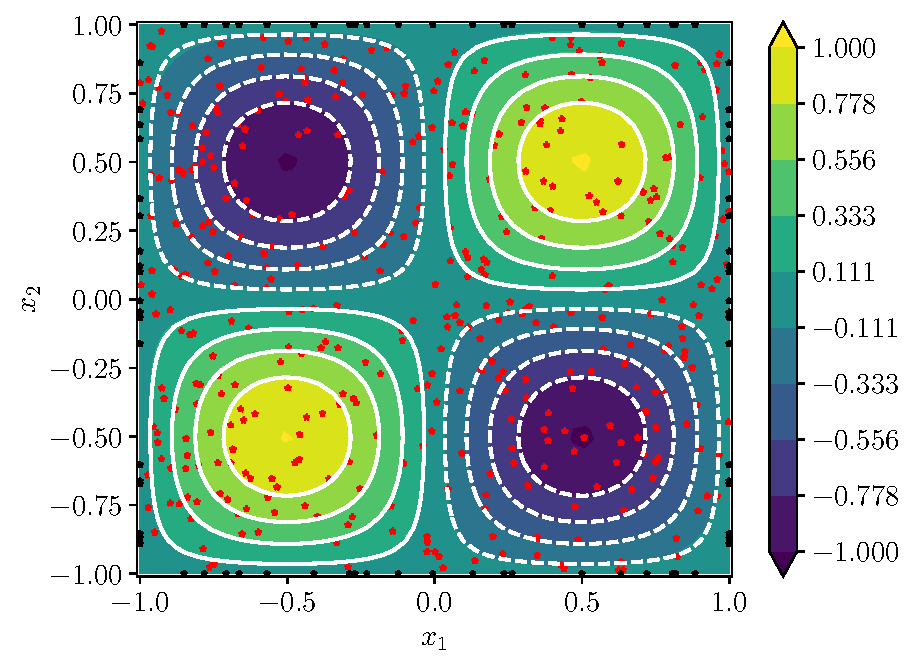
\includegraphics[width=0.8\textwidth]{cap_pinns/dados/py_pinn_poisson/fig}
  \caption{Aproximação MLP da função solução do problema de Poisson \eqref{cap_mlp_sec_eqlaplace:eq:prob}. Linhas: isolinhas da solução analítica. Mapa de cores: solução MLP. Estrelas: pontos de treinamentos na última época.}
  \label{fig:mlp_apfun_2d}
\end{figure}



\begin{lstlisting}[caption=py\_pinn\_poisson]
  import torch
  from torch import pi, sin
  
  # modelo
  nn = 50
  model = torch.nn.Sequential()
  model.add_module('layer_1', torch.nn.Linear(2,nn))
  model.add_module('fun_1', torch.nn.Tanh())
  model.add_module('layer_2', torch.nn.Linear(nn,nn))
  model.add_module('fun_2', torch.nn.Tanh())
  model.add_module('layer_3', torch.nn.Linear(nn,nn))
  model.add_module('fun_3', torch.nn.Tanh())
  model.add_module('layer_4', torch.nn.Linear(nn,1))
  
  # otimizador
  optim = torch.optim.SGD(model.parameters(),
                          lr = 1e-3, momentum=0.9)
  
  # fonte
  def f(x1, x2):
      return 2.*pi**2*sin(pi*x1)*sin(pi*x2)
  
  # treinamento
  ns_in = 400
  ns_cc = 20
  nepochs = 50000
  tol = 1e-3
  
  ## pontos de validação
  ns_val = 50
  x1_val = torch.linspace(-1., 1., steps=ns_val)
  x2_val = torch.linspace(-1., 1., steps=ns_val)
  X1_val, X2_val = torch.meshgrid(x1_val, x2_val, indexing='ij')
  X_val = torch.hstack((X1_val.reshape(ns_val**2,1),
                        X2_val.reshape(ns_val**2,1)))
  
  for epoch in range(nepochs):
      
      # forward
      X1 = 2.*torch.rand(ns_in, 1) - 1.
      X2 = 2.*torch.rand(ns_in, 1) - 1.
      X = torch.hstack((X1, X2))
      X.requires_grad = True
      
      U = model(X)
      
      # gradientes
      D1U = torch.autograd.grad(
          U, X,
          grad_outputs=torch.ones_like(U),
          retain_graph=True,
          create_graph=True)[0]
      D2UX1 =  torch.autograd.grad(
          D1U[:,0:1], X,
          grad_outputs=torch.ones_like(D1U[:,0:1]),
          retain_graph=True,
          create_graph=True)[0]
      D2UX2 =  torch.autograd.grad(
          D1U[:,1:2], X,
          grad_outputs=torch.ones_like(D1U[:,1:2]),
          retain_graph=True,
          create_graph=True)[0]
      
      # fonte
      F = f(X1, X2)
      
      # loss pts internos
      lin = torch.mean((F + D2UX1[:,0:1] + D2UX2[:,1:2])**2)
      
      # contornos
      ## c.c. 1
      X1 = 2.*torch.rand(ns_cc, 1) - 1.
      Xcc1 = torch.hstack((X1, -torch.ones((ns_cc,1))))
      Ucc1 = model(Xcc1)
      
      ## c.c. 3
      Xcc3 = torch.hstack((X1, torch.ones((ns_cc,1))))
      Ucc3 = model(Xcc3)
      
      ## c.c. 4
      X2 = 2.*torch.rand(ns_cc, 1) - 1.
      Xcc4 = torch.hstack((-torch.ones((ns_cc,1)), X2))
      Ucc4 = model(Xcc4)
      
      ## c.c. 2
      Xcc2 = torch.hstack((torch.ones((ns_cc,1)), X2))
      Ucc2 = model(Xcc2)
      
      # loss cc
      lcc = 1./(4.*ns_cc) * torch.sum(Ucc1**2 + Ucc2**2 + Ucc3**2 + Ucc4**2)
      
      # loss
      loss = lin + lcc
      
      if ((epoch % 500 == 0) or (loss.item() < tol)):
          print(f'{epoch}: loss = {loss.item():.4e}')        
  
          if (loss.item() < tol):
              break
      
      optim.zero_grad()
      loss.backward()
      optim.step()
\end{lstlisting}

% \subsection{Preprocessamento}
% [[tag:construcao]]

% Vamos assumir as seguintes mudanças de variáveis
% \begin{subequations}
%   \begin{align}
%     &\bar{x} = 2x - 1\\
%     &\bar{y} = 2y - 1.
%   \end{align}
% \end{subequations}
% Também, assumimos a notação $\bar{u}\left(\bar{\pmb{x}}\right) = u\left(\bar{\pmb{x}}(\pmb{x})\right)$.

% Então, segue que
% \begin{equation}
%   \begin{aligned}
%     \frac{\p\bar{u}}{\p\bar{x}} &= \frac{\p}{\p\bar{x}}u\left(\bar{\pmb{x}}(\pmb{x})\right)\\
%     &= \frac{\p u}{\p x}\frac{\p x}{\p \bar{x}}\\
%     &= \frac{1}{2}\frac{\p u}{\p x}.
%   \end{aligned}
% \end{equation}
% Também, temos
% \begin{equation}
%   \begin{aligned}
%     \frac{\p^2\bar{u}}{\p \bar{x}^2} &= \frac{\p}{\p\bar{x}}\left(\frac{\p\bar{u}}{\p\bar{x}}\right)\\
%     &= \frac{\p}{\p\bar{x}}\left(\frac{1}{2}\frac{\p u}{\p x}\right)\\
%     &= \frac{\p}{\p x}\left(\frac{1}{2}\frac{\p u}{\p x}\right)\frac{\p x}{\p \bar{x}}\\
%     &= \frac{1}{4}\frac{\p^2 u}{\p x^2}.
%   \end{aligned}
% \end{equation}
% Analogamente, temos
% \begin{equation}
%   \frac{\p\bar{u}}{\p\bar{y}} = \frac{1}{2}\frac{\p u}{\p y}
% \end{equation}
% e
% \begin{equation}
%   \frac{\p^2\bar{u}}{\p\bar{y}^2} = \frac{1}{4}\frac{\p^2 u}{\p y^2}.
% \end{equation}

% Na nova variável $\bar{\pmb{x}}$ o problema de Laplace \eqref{cap_mlp_sec_eqlaplace:eq:probLaplace} é equivalente a
% \begin{subequations}
%   \begin{align}
%     &\frac{\p^2\bar{u}}{\p\bar{x}^2} + \frac{\p^2\bar{u}}{\p\bar{y}^2} = 0, ~\bar{\pmb{x}}=(\bar{x}, \bar{y})\in (-1, 1)^2,\\
%     &\bar{u} = \bar{u}_0, ~\bar{\pmb{x}}\in\Gamma=\p D.
%   \end{align}
% \end{subequations}

% \begin{ex}
% \begin{lstlisting}[caption=pyEqLaplacePP]
% import torch
% import matplotlib.pyplot as plt
% import random
% import numpy as np

% # modelo
% ## n camadas escondidas
% nh = 3
% ## n neurônios por camada
% nn = 50
% ## fun de ativação
% fh = torch.nn.Tanh()
% ## arquitetura
% model = torch.nn.Sequential()
% model.add_module('layer_1', torch.nn.Linear(2,nn))
% model.add_module('fun_1', fh)
% for layer in range(2, nh):
%     model.add_module(f'layer_{layer}', torch.nn.Linear(nn,nn))
%     model.add_module(f'fun_{layer}', fh)
% model.add_module(f'layer_{nh}', torch.nn.Linear(nn,1))

% # SGD - (Stochastic) Gradient Descent
% optim = torch.optim.SGD(model.parameters(),
%                         lr = 1e-2,
%                         momentum = 0.9)
% optim = torch.optim.Adam(model.parameters(),
%                         lr = 1e-2)

% # params treinamento
% ## n épocas
% nepochs = 10001
% ## freq output loss
% nout_loss = 100
% ## stop criterion
% tol = 1e-4

% ## n amostras por eixo
% ns = 101

% lloss = []
% for epoch in range(nepochs):

%     # forward
    
%     ## internal pts samples
%     Xin = 2.*torch.rand((ns, 2)) -1.
%     Xin.requires_grad=True
%     Uin = model(Xin)

%     ## loss internal pts
%     D1Uin = torch.autograd.grad(
%         Uin, Xin,
%         grad_outputs=torch.ones_like(Uin),
%         retain_graph=True,
%         create_graph=True)[0]
%     D2Uin = torch.autograd.grad(
%         D1Uin, Xin,
%         grad_outputs=torch.ones_like(D1Uin),
%         retain_graph=True,
%         create_graph=True)[0]

%     lin = torch.mean((D2Uin[:,0] + D2Uin[:,1])**2)

%     ## bc 1
%     xx = 2.*torch.rand((ns, 1)) - 1.
%     yy = -1.*torch.ones((ns,1))
%     Xbc1 = torch.hstack((xx, yy))
%     Ubc1 = model(Xbc1)

%     ## loss bc 1
%     xx = (xx + 1.)/2.;
%     Uexp = xx*(1. - xx)
%     lbc1 = torch.mean((Ubc1 - Uexp)**2)

%     ## bc 3
%     xx = 2.*torch.rand((ns, 1)) -1.
%     yy = torch.ones((ns,1))
%     Xbc3 = torch.hstack((xx, yy))
%     Ubc3 = model(Xbc3)

%     ## loss bc 3
%     xx = (xx + 1.)/2.;
%     Uexp = xx*(1. - xx)
%     lbc3 = torch.mean((Ubc3 - Uexp)**2)

%     ## bc 2
%     xx = torch.ones((ns, 1))
%     yy = 2.*torch.rand((ns,1)) -1.
%     Xbc2 = torch.hstack((xx, yy))
%     Ubc2 = model(Xbc2)

%     ## loss bc 2
%     yy = (yy + 1.)/2.;
%     Uexp = yy*(yy - 1.)
%     lbc2 = torch.mean((Ubc2 - Uexp)**2)

%     ## bc 4
%     xx = -1.*torch.ones((ns, 1))
%     yy = 2.*torch.rand((ns,1)) -1.
%     Xbc4 = torch.hstack((xx, yy))
%     Ubc4 = model(Xbc4)

%     ## loss bc 3
%     yy = (yy + 1.)/2.;
%     Uexp = yy*(yy - 1.)
%     lbc4 = torch.mean((Ubc4 - Uexp)**2)

%     # loss function
%     loss = lin + lbc1 + lbc2 + lbc3 + lbc4

%     lloss.append(loss.item())

%     if (((epoch % nout_loss) == 0) or (loss.item() < tol)):
%         print(f'{epoch}: loss = {loss.item():.4e}')
    
%         # gráfico
%         fig = plt.figure()
%         ax = fig.add_subplot()

%         npts = 50
%         xx = torch.linspace(-1., 1., npts)
%         yy = torch.linspace(-1., 1., npts)
%         X, Y = torch.meshgrid(xx, yy)
%         # exact
%         Uexp = (X+1.)/2.*(1. - (X+1.)/2.) \
%             - (Y+1.)/2.*(1. - (Y+1.)/2.)
%         c = ax.contour(X, Y, Uexp, levels=10, colors='white')
%         ax.clabel(c)

%         M = torch.hstack((X.reshape(-1,1),
%                           Y.reshape(-1,1)))
%         Uest = model(M).detach()
%         Uest = Uest.reshape((npts, npts))
%         cf = ax.contourf(X, Y, Uest, levels=10, cmap='coolwarm')
%         plt.colorbar(cf)
        
%         ax.grid()
%         ax.set_xlabel('$\\bar{x}$')
%         ax.set_ylabel('$\\bar{y}$')
%         plt.title(f"epoch = {epoch}, loss = {loss.item():.4e}")
%         plt.savefig(f'results/sol_{epoch:0>6}.png', bbox_inches='tight')
%         plt.close()

%     if (loss.item() < tol):
%         break

%     # backward
%     optim.zero_grad()
%     loss.backward()
%     optim.step()

% fig = plt.figure()
% ax = fig.add_subplot()
% ax.plot(lloss)
% ax.set_yscale('log')
% plt.show()
% \end{lstlisting}
% \end{ex}

% \subsection{Diferenças Finitas}

% % \lstinputlisting[caption=mlp\_eqlaplace.py, label=cap_mlp_sec_modelo:cod:mlp_eqlaplace]{./cap_mlp/dados/py_mlp_eqlaplace/main.py}
% \begin{lstlisting}[caption=mlp\_eqlaplace\_df.py, label=cap_mlp_sec_modelo:cod:mlp_eqlaplace_df]
% import torch
% import matplotlib.pyplot as plt
% import random
% import numpy as np

% # modelo
% model = torch.nn.Sequential(
%     torch.nn.Linear(2,50),
%     torch.nn.Tanh(),
%     torch.nn.Linear(50,10),
%     torch.nn.Tanh(),
%     torch.nn.Linear(10,5),
%     torch.nn.Tanh(),
%     torch.nn.Linear(5,1)
% )

% # SGD - (Stochastic) Gradient Descent
% optim = torch.optim.SGD(model.parameters(),
%                         lr = 1e-3,
%                         momentum = 0.9,
%                         dampening = 0.)

% # Solução esperada
% def u(x, y):
%     return a*x*(1-x) - a*y*(1-y)


% def laplace_loss(X, U, h2, n, uc=u, p=1.):
%     # num de amostras
%     nc = 2*n + 2*(n-2)
%     ni = n**2 - nc

%     # loss interno
%     lin = 0.
%     for i in range(1,n-1):
%       for j in range(1,n-1):
%         s = j + i*n
%         l = (U[s-n, 0] - 2 * U[s, 0] + U[s+n, 0])/h2 # x
%         l += (U[s-1, 0] - 2 * U[s, 0] + U[s+1, 0])/h2 # y
%         lin += l**2
%     lin /= ni 

%     # loss contorno
%     lc = 0.
%     # 0 <= x <= 1 e y == 0
%     for i in range(n):
%         s = i*n
%         x = M[s,0]
%         y = M[s,1]
%         lc += (U[s,0] - uc(x,y))**2
%     # 0 <= x <= 1 e y == 1
%     for i in range(n):
%         s = n-1 + i*n
%         x = M[s,0]
%         y = M[s,1]
%         lc += (U[s,0] - uc(x,y))**2
%     # 0 == x e 0 < y < 1
%     for j in range(1, n-1):
%         s = j
%         x = M[s,0]
%         y = M[s,1]
%         lc += (U[s,0] - uc(x,y))**2
%     # 1 == x e 0 < y < 1
%     for j in range(1, n-1):
%         s = j + n*(n-1)
%         x = M[s,0]
%         y = M[s,1]
%         lc += (U[s,0] - uc(x,y))**2
%     lc *= p/nc
    
%     loss = lin + lc
%     return loss

    
% # dados do problema

% # collocation points
% a = 1
% n = 11
% ns = n**2
% h = 1./(n-1)
% h2 = h**2

% # malha
% x = torch.linspace(0, 1, n)
% y = torch.linspace(0, 1, n)

% M = torch.empty((ns, 2))
% s = 0
% for i, xx in enumerate(x):
%   for j, yy in enumerate(y):
%     M[s,0] = xx
%     M[s,1] = yy
%     s += 1

% # gráfico
% X, Y = np.meshgrid(x, y)
% U_esp = u(X, Y)

% # training
% nepochs = 10000
% nout_loss = 100
% nout_plot = 500

% for epoch in range(nepochs):

%     # forward
%     U_est = model(M)

%     # loss function
%     loss = laplace_loss(M, U_est, h2, n, u, p=10.)

%     if ((epoch % nout_loss) == 0):
%         print(f'{epoch}: loss = {loss.item():.4e}')
    
%     # output current solution
%     if ((epoch) % nout_plot == 0):
%         # verificação
%         fig = plt.figure()
%         ax = fig.add_subplot()

%         ns = 50
%         x1 = torch.linspace(0., 1., ns)
%         x2 = torch.linspace(0., 1., ns)
%         X1, X2 = torch.meshgrid(x1, x2)
%         # exact
%         Z_esp = torch.empty_like(X1)
%         for i,x in enumerate(x1):
%             for j,y in enumerate(x2):
%                 Z_esp[i,j] = u(x, y)
%         c = ax.contour(X1, X2, Z_esp, levels=10, colors='white')
%         ax.clabel(c)

%         X_plot = torch.cat((X1.reshape(-1,1),
%                             X2.reshape(-1,1)), dim=1)
%         Z_est = model(X_plot)
%         Z_est = Z_est.reshape((ns,ns))
%         cf = ax.contourf(X1, X2, Z_est.detach(), levels=10, cmap='coolwarm')
%         plt.colorbar(cf)
        
%         ax.grid()
%         ax.set_xlabel('$x_1$')
%         ax.set_ylabel('$x_2$')
%         plt.show()        

%     # backward
%     optim.zero_grad()
%     loss.backward()
%     optim.step()
% \end{lstlisting}

\subsection{Exercícios}

\begin{exer}
  Crie uma MLP para resolver
  \begin{align}
    &-\Delta u = 0, ~\pmb{x}\in D = (0, 1)^2,\\
    &u(x_1, 0) = x1(1-x_1), 0 \leq x_1 \leq 1,\\
    &u(1, x_2) = x2(1-x_2), 0 < x_2 \leq 1,\\
    &u(x_1, 1) = x1(1-x_1), 0 \leq x_1 < 1,\\
    &u(0, x_2) = x2(1-x_2), 0 < x_2 < 1.
  \end{align}
\end{exer}
\begin{resp}
  Dica: solução analítica $u(x_1, x_2) = x_1(1-x_1) - x_2(1-x_2)$.
\end{resp}

\section{Aplicação: Equação do Calor}\label{cap_mlp_sec_calor}
\badgeConstrucao

Consideramos o problema
\begin{subequations}\label{cap_mlp_sec_calor:eq:prob}
  \begin{align}
    &u_t = u_{xx} + f, (t,x)\in (0, 1] \times (-1, 1),\\
    &u(0,x) = \sen(\pi x), x\in [-1, 1],\\
    &u(t,-1) = u(t,1) = 0, t\in (t_0, tf],
  \end{align}
\end{subequations}
onde $f(t,x) = (\pi^2 - 1)e^{-t}\sen(\pi x)$ é a fonte. Este problema foi manufaturado a partir da solução
\begin{equation}
  u(t,x) = e^{-t}\sen(\pi x).
\end{equation}

\begin{lstlisting}[caption=mlp\_calor\_autograd.py]
import torch
from torch import pi, sin, exp
from collections import OrderedDict
import matplotlib.pyplot as plt

# modelo
hidden = [50]*8
activation = torch.nn.Tanh()
layerList = [('layer_0', torch.nn.Linear(2, hidden[0])),
             ('activation_0', activation)]
for l in range(len(hidden)-1):
    layerList.append((f'layer_{l+1}',
                      torch.nn.Linear(hidden[l], hidden[l+1])))
    layerList.append((f'activation_{l+1}', activation))
layerList.append((f'layer_{len(hidden)}', torch.nn.Linear(hidden[-1], 1)))
#layerList.append((f'activation_{len(hidden)}', torch.nn.Sigmoid()))
layerDict = OrderedDict(layerList)
model = torch.nn.Sequential(OrderedDict(layerDict))

# otimizador
# optim = torch.optim.SGD(model.parameters(),
#                          lr = 1e-3, momentum=0.85)
optim = torch.optim.Adam(model.parameters(),
                         lr = 1e-2)
scheduler = torch.optim.lr_scheduler.ReduceLROnPlateau(optim,
                                                       factor=0.1,
                                                       patience=100)

# treinamento
nt = 10
tt = torch.linspace(0., 1., nt+1)
nx = 20
xx = torch.linspace(-1., 1., nx+1)
T,X = torch.meshgrid(tt, xx, indexing='ij')
tt = tt.reshape(-1,1)
xx = xx.reshape(-1,1)

Sic = torch.hstack((torch.zeros_like(xx), xx))
Uic = sin(pi*xx)

Sbc0 = torch.hstack((tt[1:,:], -1.*torch.ones_like(tt[1:,:])))
Ubc0 = torch.zeros_like(tt[1:,:])

Sbc1 = torch.hstack((tt[1:,:], 1.*torch.ones_like(tt[1:,:])))
Ubc1 = torch.zeros_like(tt[1:,:])

tin = tt[1:,:]
xin = xx[1:-1,:]
Sin = torch.empty((nt*(nx-1), 2))
Fin = torch.empty((nt*(nx-1), 1))
s = 0
for i,t in enumerate(tin):
    for j,x in enumerate(xin):
        Sin[s,0] = t
        Sin[s,1] = x
        Fin[s,0] = (pi**2 - 1.)*exp(-t)*sin(pi*x)
        s += 1
tin = torch.tensor(Sin[:,0:1], requires_grad=True)
xin = torch.tensor(Sin[:,1:2], requires_grad=True)
Sin = torch.hstack((tin,xin))

nepochs = 50001
tol = 1e-4
nout = 100

for epoch in range(nepochs):

    # loss

    ## c.i.
    Uest = model(Sic)
    lic = torch.mean((Uest - Uic)**2)
    
    ## residual
    U = model(Sin)
    U_t = torch.autograd.grad(
        U, tin,
        grad_outputs=torch.ones_like(U),
        retain_graph=True,
        create_graph=True)[0]
    U_x = torch.autograd.grad(
        U, xin,
        grad_outputs=torch.ones_like(U),
        retain_graph=True,
        create_graph=True)[0]
    U_xx = torch.autograd.grad(
        U_x, xin,
        grad_outputs=torch.ones_like(U_x),
        retain_graph=True,
        create_graph=True)[0]
    res = U_t - U_xx - Fin
    lin = torch.mean(res**2)

    ## c.c. x = -1
    Uest = model(Sbc0)
    lbc0 = torch.mean(Uest**2)

    ## c.c. x = 1
    Uest = model(Sbc1)
    lbc1 = torch.mean(Uest**2)

    loss = lin + lic + lbc0 + lbc1

    lr = optim.param_groups[-1]['lr']
    print(f'{epoch}: loss = {loss.item():.4e}, lr = {lr:.4e}')

    # backward
    scheduler.step(loss)
    optim.zero_grad()
    loss.backward()
    optim.step()


    # output
    if ((epoch % nout == 0) or (loss.item() < tol)):
        plt.close()
        fig = plt.figure(dpi=300)
        nt = 10
        tt = torch.linspace(0., 1., nt+1)
        nx = 20
        xx = torch.linspace(-1., 1., nx+1)
        T,X = torch.meshgrid(tt, xx, indexing='ij')
        Uesp = torch.empty_like(T)
        M = torch.empty(((nt+1)*(nx+1),2))
        s = 0
        for i,t in enumerate(tt):
            for j,x in enumerate(xx):
                Uesp[i,j] = exp(-t)*sin(pi*x)
                M[s,0] = t
                M[s,1] = x
                s += 1
        Uest = model(M)
        Uest = Uest.detach().reshape(nt+1,nx+1)
        l2rel = torch.norm(Uest - Uesp)/torch.norm(Uesp)
        
        ax = fig.add_subplot()
        cb = ax.contourf(T, X, Uesp,
                         levels=10)
        fig.colorbar(cb)
        cl = ax.contour(T, X, Uest,
                        levels=10, colors='white')
        ax.clabel(cl, fmt='%.1f')
        ax.set_xlabel('$t$')
        ax.set_ylabel('$x$')
        plt.title(f'{epoch}: loss = {loss.item():.4e}, l2rel = {l2rel:.4e}')
        plt.savefig(f'./results/sol_{(epoch//nout):0>6}.png')

    if ((loss.item() < tol) or (lr < 1e-6)):
        break
\end{lstlisting}


\section{PINN com Parâmetro a Determinar}\label{cap_pinns_sec_param}
\badgeConstrucao

Vamos considerar uma \hlemph{equação diferencial}
\begin{equation}\label{cap_pinns_sec_param:eq:ed}\hleq
  L(u;\lambda) = f, ~\pmb{x}\in D\subset\mathbb{R}^n,
\end{equation}
onde $L$ é um operador em funções $u = u(\pmb{x})$, $\lambda\in\mathbb{R}$ é um \hlemph{parâmetro a determinar} e $f$ uma dada função fonte. Assumimos conhecidas condições inicial e de contorno, bem como um \hlemph{conjunto de amostras}
\begin{equation}\hleq
  \mathcal{D} := \left\{\left(\pmb{x}^{(s)},u^{(s)}\right)\right\}_{s=1}^{n_s},
\end{equation}
com $\pmb{x}^{(s)}\in D$ e $u^{(s)} = u\left(\pmb{x}^{(s)}\right)$.

Uma rede informada pela física (\hlemph{PINN}, do inglês, \textit{Physics-informed neural network}) \hlemph{com parâmetro a determinar} é uma rede neural
\begin{equation}\hleq
  \tilde{u} = \mathcal{N}(\pmb{x};\lambda),
\end{equation}
em que $\tilde{u}$ é a solução estimada do modelo dado pela equação diferencial \eqref{cap_pinns_sec_param:eq:ed} com dadas condições inicial e de contorno, em que \hl{o parâmetro $\lambda$ é estimado tal que}
\begin{equation}
  \tilde{u}^{(s)} \approx u^{(s)}, ~\left(\pmb{x}^{(s)},u^{(s)}
\right)\in\mathcal{D}.
\end{equation}

\begin{figure}[H]
  \centering
  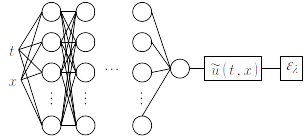
\includegraphics[width=0.8\textwidth]{cap_pinns/dados/fig_pinns_param/fig}
  \caption{Esquema de uma PINN $\tilde{u} = \mathcal{N}(\pmb{x};\lambda)$.}
  \label{cap_pinns_sec_param:fig:pinn}
\end{figure}

Considerando uma rede do tipo perceptron multicamadas (MLP, do inglês, \textit{multilayer perceptron}, consulte Fig.~\ref{cap_pinns_sec_param:fig:pinn}), seus pesos e \textit{biases} são treinados em conjunto com parâmetro $\lambda$ de forma a minimizar a \hlemph{função de perda}
\begin{equation}
  \begin{aligned}
    &{\color{blue}\varepsilon_\lambda := \underbrace{\frac{1}{n_{\text{in}}}\sum_{s=1}^{n_{\text{in}}}\left|\mathcal{R}_\lambda\left(\pmb{x}_{\text{in}}^{(s)}\right)\right|^2}_{\text{pts. internos}}}\\
    &{\color{blue}\quad + \underbrace{\frac{1}{n_{\text{cc}}}\sum_{s=1}^{n_{\text{cc}}}\left|\tilde{u}_{\text{cc}}-u_{\text{cc}}\right|^2}_{\text{c.i. \& c.c.}}}\\
    &{\color{red}\quad + \underbrace{\frac{p}{n_s}\sum_{s=1}^{n_s}\left|\tilde{u}^{(s)}-u^{(s)}\right|^2}_{\text{amostras}}},
  \end{aligned}
\end{equation}
onde $p\geq 0$ é uma \emph{penalidade} e
\begin{equation}
  \mathcal{R}_\lambda(\pmb{x}) := f - L(u;\lambda)
\end{equation}
é o \emph{resíduo} de \eqref{cap_pinns_sec_param:eq:ed}.

\begin{ex}\label{cap_pinns_sec_param:ex:fisher}
  Consideramos a equação de Fisher{\fisher}
  \begin{equation}
    u_t = u_{xx} + \lambda u(1-u), ~(t,x)\in(0,t_f)\times(0,1),
  \end{equation}
  com o parâmetro $\lambda>0$ a determinar. Assumimos dadas condição inicial
  \begin{equation}
    u(0,x) = \frac{1}{\left(1+e^{\sqrt{\frac{\lambda}{6}}x}\right)^2}, ~x\in[0,1],
  \end{equation}
  e condições de contorno
  \begin{align}
    &u_x(t,0) = \frac{1}{\left(1+e^{-\frac{5}{6}\lambda t}\right)^2},\\
    &u_x(t,0) = \frac{1}{\left(1+e^{\sqrt{\frac{\lambda}{6}}-\frac{5}{6}\lambda t}\right)^2}.
  \end{align}
  
  Este problema tem solução analítica \cite{Agirseven2010a}
  \begin{equation}
    u_a(t,x) = \frac{1}{\left(1+e^{\sqrt{\frac{\lambda}{6}}x-\frac{5}{6}\lambda t}\right)^2}.
  \end{equation}

  Como exemplo de aplicação de uma PINN com parâmetro a determinar, vamos assumir o seguinte conjunto de amostras
  \begin{equation}
    \mathcal{D} = \left\{\left(\left(t^{(s)},x^{(s)}\right),u^{(s)}\right)\right\}_{s=1}^{n_s},
  \end{equation}
  com $\left(t^{(s)},x^{(s)}\right)\in\{0.1, 0.2, 0.3\}\times\{0.25,0.5,0.75\}$ e $u^{(s)} = u_a\left(t^{(s)},x^{(s)}\right)$.

  \begin{figure}[H]
    \centering
    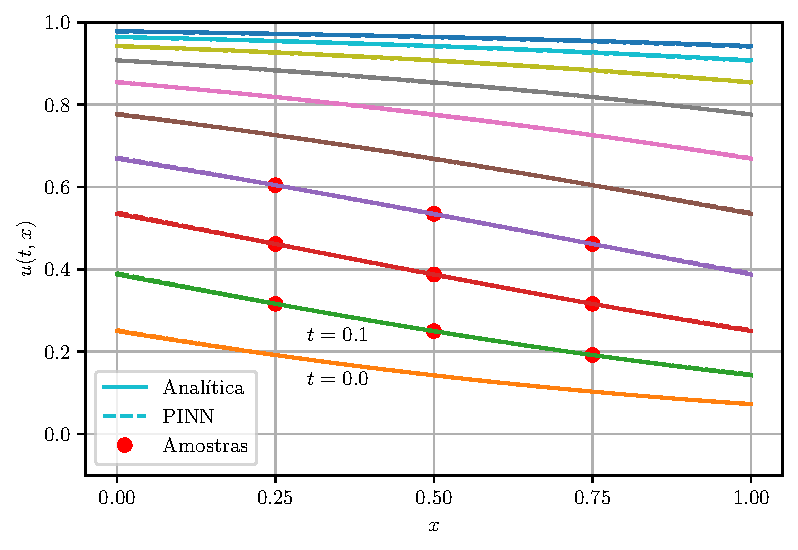
\includegraphics[width=0.8\textwidth]{cap_pinns/dados/ex_pinn_fisher/fig}
    \caption{Solução PINN \textit{versus} analítica para $\lambda = 6$.}
  \end{figure}

\begin{lstlisting}[caption=ex\_pinn\_fisher.py]
import torch

# modelo
nh = 4
nn = 50
fun = torch.nn.Tanh()
model = torch.nn.Sequential()
model.add_module('layer_1', torch.nn.Linear(2, nn))
model.add_module('fun_1', fun)
for l in range(2, nh+1):
    model.add_module(f'layer_{l}', torch.nn.Linear(nn, nn))
    model.add_module(f'fun_{l}', fun)
model.add_module(f'layer_{nh+1}', torch.nn.Linear(nn, 1))

# parâmetro
rgn = [5., 7]
model.lmbda = torch.nn.Parameter(
    data=(rgn[1]-rgn[0])*torch.rand(1)+rgn[0])

# otimizador
optim = torch.optim.Adam(model.parameters(), lr=0.001)

# parâmetros do problema
tf = 1.

# solução analítica
lmbda = torch.tensor([6.])
def ua(t,x, lmbda=lmbda):
    return 1./(1.+torch.exp(torch.sqrt(lmbda/6.)*x-5./6*lmbda*t))**2

# condição inicial
def u0(x, lmbda=lmbda):
    return 1./(1.+torch.exp(torch.sqrt(lmbda/6)*x))**2

# amostras
ts = torch.tensor([0.1, 0.2, 0.3])
xs = torch.tensor([0.25, 0.5, 0.75])
T, X = torch.meshgrid(ts, xs, indexing='ij')
Ss = torch.hstack((T.reshape(-1,1), X.reshape(-1,1)))
Us_exp = ua(T, X).reshape(-1,1)

# treinamento
nepochs = 50000
tol = 1e-5

eout = 100

sin = 50
penalty = 1e1

for epoch in range(nepochs):

    # forward

    ## pts internos
    tsin = tf*torch.rand(sin, 1)
    xsin = torch.rand(sin, 1)
    Sin = torch.hstack((tsin, xsin))
    Sin.requires_grad = True

    Uin = model(Sin)

    ## loss pts internos
    DUin = torch.autograd.grad(
        Uin, Sin, 
        torch.ones_like(Uin), 
        create_graph=True,
        retain_graph=True)[0]
    Uin_t = DUin[:,0:1]
    Uin_x = DUin[:,1:2]

    Uin_xx = torch.autograd.grad(
        Uin_x, Sin,
        torch.ones_like(Uin_x),
        create_graph=True,
        retain_graph=True)[0][:,1:2]
    
    
    lin = torch.mean((Uin_t - Uin_xx \
                      - model.lmbda*Uin*(1-Uin))**2)
    
    ## cond. inicial
    S0 = torch.hstack((torch.zeros_like(xsin), xsin))

    U0 = model(S0)

    ## loss cond. inicial
    l0 = torch.mean((U0 - u0(xsin))**2)

    ## cond. de contorno
    Sbc0 = torch.hstack((tsin, torch.zeros_like(xsin)))
    Sbc1 = torch.hstack((tsin, torch.ones_like(xsin)))
    Sbc = torch.vstack((Sbc0, Sbc1))

    Ubc_exp = ua(Sbc[:,0:1],Sbc[:,1:2])
    Ubc_est = model(Sbc)

    ## loss cond. de contorno    
    lbc = torch.mean((Ubc_est - Ubc_exp)**2)

    ## amostras
    Us_est = model(Ss)

    ## loss amostras
    ls = torch.mean((Us_est - Us_exp)**2)

    ## loss total
    loss = lin + l0 + lbc + penalty*ls 

    if ((epoch % eout == 0) or (loss.item() < tol)):
        print(f'epoch: {epoch}, '\
              + f'loss={loss.item():.4e}, '\
              + f'lmbda={model.lmbda.item():.3f}')
    
    if (loss.item() < tol):
        break
        
    optim.zero_grad()
    loss.backward()
    optim.step()  
\end{lstlisting}
\end{ex}

\subsection{Exercícios}
\badgeConstrucao

\begin{ex}
  Considere o seguinte problema de valor inicial
  \begin{subequations}
    \begin{align}
      &-u'' = \lambda\sen(\pi x), ~0<x<1,\\
      &u(0) = u(1) = 0,
    \end{align}
  \end{subequations}
  onde $\lambda>0$ é um parâmetro a determinar. Dadas as amostras
  \begin{equation}
    \mathcal{D} = \left\{\left(\frac{1}{6},\frac{1}{2}\right), \left(\frac{1}{4},\sqrt{2}{2}\right), \left(\frac{1}{3},\sqrt{3}{3}\right)\right\},
  \end{equation}
  crie uma PINN 
  \begin{equation}
    \tilde{u} = \mathcal{N}(x;\lambda) 
  \end{equation}
  para estimar o parâmetro $\lambda$ e a solução em todo o domínio $0\leq x\leq 1$.
\end{ex}
\begin{resp}
  $\lambda = \pi^2$
\end{resp}

\begin{ex}
  Considere o problema de Poisson{\poisson}
  \begin{subequations}
    \begin{align}
      &-\nabla u = \lambda, ~(x,y)\in D=(-1,1)^2,\\
      &u = 0, (x,y)\in\p D,        
    \end{align}
  \end{subequations}
  onde $\lambda > 0$ é um parâmetro a determinar. Dado que $u(1/2,1/2) = 1/8$, crie uma PINN 
  \begin{equation}
    \tilde{u} = \mathcal{N}(x,y;\lambda)
  \end{equation}
  para estimar o parâmetro $\lambda$ e a solução em todo o domínio $D$.
\end{ex}
\begin{resp}
  $\lambda = 1$
\end{resp}

\begin{ex}
  Considere o problema de calor
  \begin{subequations}
    \begin{align}
      &u_t = \lambda u_{xx} + (\pi^2-1)e^{-t}\sen(\pi x), ~(t,x)\in(0,1)^2,\\
      &u(0,x) = \sen(\pi x), ~x\in[0,1],\\
      &u(t,0) = u(t,1) = 0, ~t\in[0,1],
    \end{align}
  \end{subequations}
  onde o coeficiente de difusão $\lambda>0$ é um parâmetro a determinar. Sabendo que o problema tem solução analítica
  \begin{equation}
    u(t,x) = e^{-t}\sen(\pi x),
  \end{equation}
  escolha um conjunto de amostras $\mathcal{D} = \left\{\left(\left(t^{(s)},x^{(s)}\right),u^{(s)}\right)\right\}_{s=1}^{n_s}$ tal que seja possível estimar $\lambda$ com uma PINN
  \begin{equation}
    \tilde{u} = \mathcal{N}(t,x;\lambda).
  \end{equation}
\end{ex}
\begin{resp}
  $\lambda = 1$
\end{resp}

% \begin{ex}
%   Considere o problema de Burgers{\burgers}
%   \begin{subequations}
%     \begin{align}
%       &u_t + uu_x = \lambda u_{xx}, ~(t,x)\in(0,1)^2,\\
%       &u(0,x) = 4\pi\frac{\sen(\pi x)}{2+\cos(\pi x)}, ~x\in(0,1),\\
%       &u(t,0)=u(t,1)=0, ~t\in(0,1),
%     \end{align}
%     com coeficiente de difusão $\lambda>0$ a determinar. 
%   \end{subequations}
% \end{ex}